\chapter{Professional Growth}
\begin{flushleft}


\label{ch:results}

Presenting found literature in a useful way

\section{Technology and Tools I Learned}
As Orbitax develops its tools in various technologies. As an intern, I saw them very closely and I had the privilege to learn some of technologies. 


\subsection{Tools}
Programming tools make development easier. In my Intern at Orbitax I have to use the following tools in my daily works:

\begin{itemize}
    \item Webstorm
    \item Visual studio code
    \item React native debugger
    \item Android studio
    \item Xcode
    \item Android and IOS Emulator
    \item Postman
    \item Sublime merge
\end{itemize}

\subsection{Technology}
\subsubsection{RxJs}
RxJS is a library for composing asynchronous and event-based programs by using observable sequences. Think of RxJS as Lodash for events. It’s Reactive Extensions for JavaScript.

 \begin{figure}[htbp]
\centerline{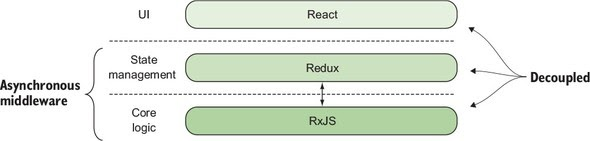
\includegraphics[scale=0.5]{Figures/react.jpg}}
\caption{Layered diagram of the 3R architecture that shows the hierarchy of the different layers of the system}
\label{fig}
\end{figure}

\subsubsection{Redux}
While Redux can be used with any UI layer, it was originally designed and intended for use with React. There are UI binding layers for many other frameworks, but React-Redux is maintained directly by the Redux team.

As the official Redux binding for React, React-Redux is kept up-to-date with any API changes from either library, to ensure that your React components behave as expected. Its intended usage adopts the design principles of React - writing declarative components.

\subsubsection{React Native}
This is a framework for native applications. React Native runs on React, a popular open-source library for building user interfaces with JavaScript. To make the most of React Native, it helps to understand React itself. This section can get you started or can serve as a refresher course.

 \begin{figure}[htbp]
\centerline{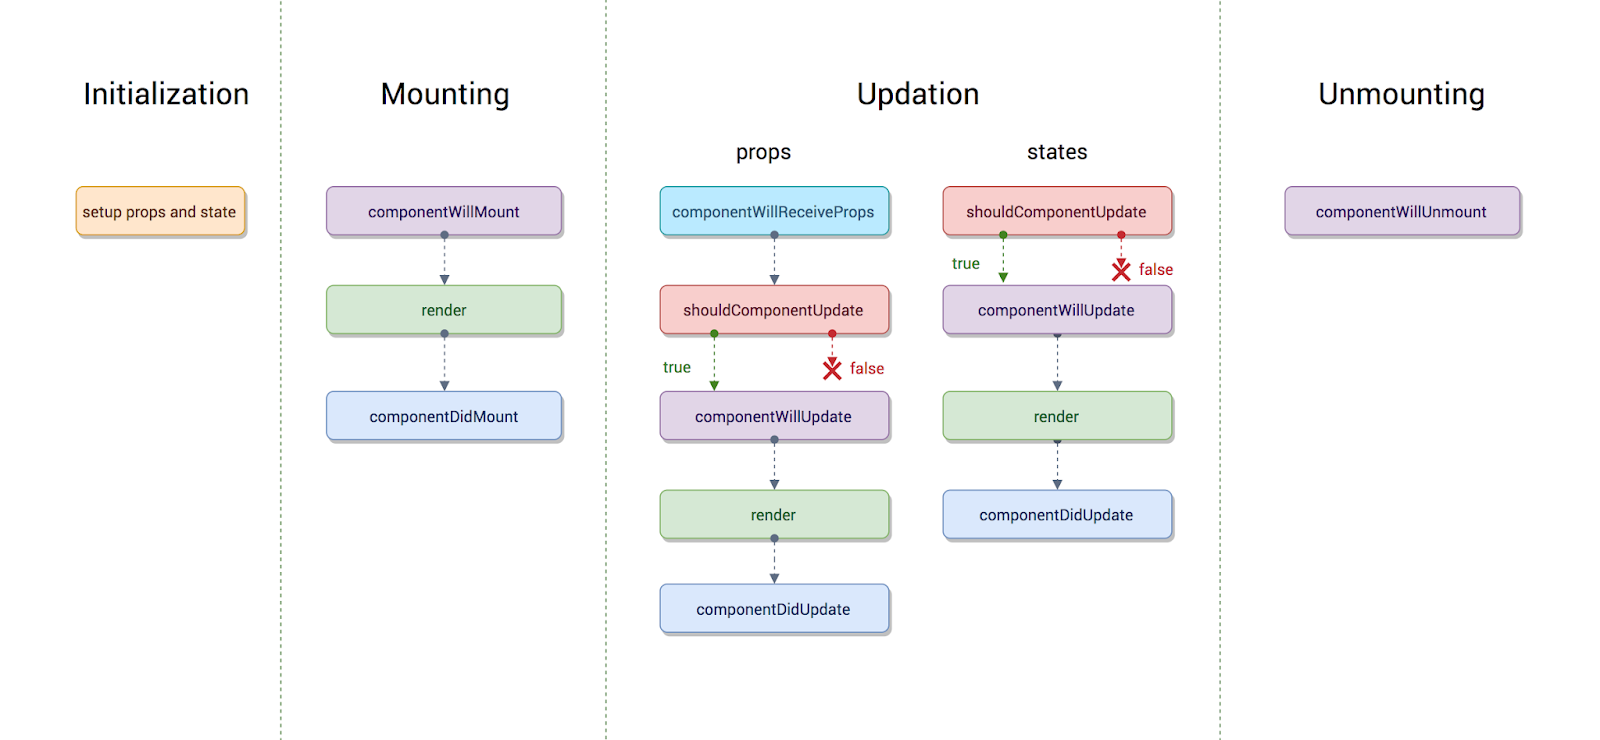
\includegraphics[scale=0.3]{Figures/component.png}}
\caption{React native Component Lifecycle}
\label{fig}
\end{figure}


\section{Development Technique, Pair Programming}
In the Internship, I had the privilege to understand pair-programming perfectly. As I was new to the Orbitax ecosystem, I always had a lot of questions. Therefore, I could clear my confusion while talking with the seniors and gain knowledge about the platform.
Actually, in varsity, we always worked as a team. But never did actual teamwork. In Orbitax, I learned about actual teamwork. Where some developer works in a different part of the same applications.
While working as a pair, we used to work in a way, when my partner was typing I was assisting him, giving him ideas and checking for mistakes; when I was typing my partner was giving me instructions.
Here in Orbitax, I learned that this is an agile programming technique known as Pair Programming. \\
\textit{“Pair programming is an agile software development technique in which two programmers work together at one workstation. One, the driver, types in code while the other, the observer (or navigator), reviews each line of code as it is typed in. The two programmers switch roles frequently.”} \\ 
In Orbitax pair programming is done most of the time and it works as a real technique. Although pair programming is not suitable in all situations, I believe some situations are the most perfect situation for paired programming which are recognized by my experienced team members.

 \begin{figure}[htbp]
\centerline{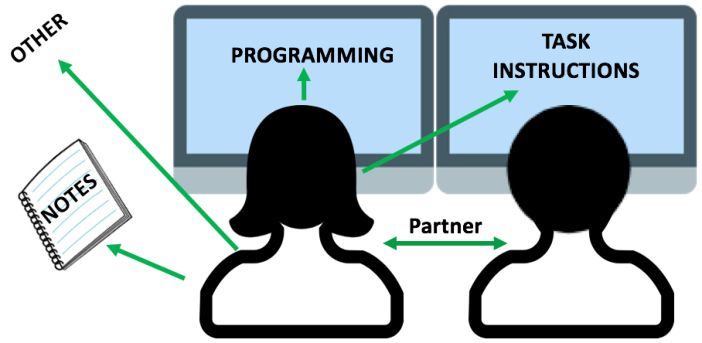
\includegraphics[scale=0.3]{Figures/p.png}}
\caption{Pair Programming}
\label{fig}
\end{figure}

\subsection{Benefits and Costs of pair programming}
Some studies suggest that pair programming produces software with fewer bugs than software developed alone. Reduction in defect rates of 15 percent to 50 percent, varying depending on programmer experience and task complexity. Pairs typically find more design alternatives than programmers working alone, and arrive at simpler, more-maintainable design; they also catch design defects early. Pairs usually complete work faster than one programmer assigned to the same task. \\ 

However, some other studies suggest that pair programming is not uniformly beneficial or effective because although it produces faster, the total programmer time in pair programming is usually higher than that of programming alone.



\section{Professional Learning}
Although technical learning is important, professional learning is the sole purpose of an internship. Orbitax is an excellent place to learn professionalism.

\subsection{No bullying and blaming}
Software development is always teamwork. And in a team, all members don't have similar skills or knowledge. This is true for Orbitax too. During my time of internship, I have made many mistakes like did not maintain code structure. And sometimes stuck in a problem for many hours. But my team leader had never been harsh with me. He always encouraged me to ask for help when I was stuck for some hour. But he did not solve the problem himself unless it was necessary. He always suggests an approach for how to solve that problem. He always encourages us to dig into the error. \\ 
In Orbitax,  I have never seen team leaders and project managers bully people working under their supervision.  \\ 
This practice is effective to keep the work environment healthy. Blaming others for their mistakes does not solve the problem. It only makes the situation and the relationship between coworkers worse.



\subsection{Always Complete your work}
At Orbitax, Everyone is assigned to a particular work and he does his work in his way. At times of scrum, everyone shares their progress with others. All the projects are done in this way. 

\subsection{ Appreciate success, do not discourage for failure}
 The team I have been assigned to has taught me the value of appreciation. Here, the members appreciate each other on their successful contribution to the company and also on their success in some other fields.  
The employees do not discourage people from failure in a particular task. People who can have expertise in that field help others. \\ 
Orbitax gives time to its employees to learn and work at the same time. It has a really good work environment.

\subsection{Attiude}
Orbitax Ltd. is a Software Company with full of fun and creative and Orbitaxians are very much friendly. As an intern, these attract me very much and I always try to follow them to be a successful Software Engineer as well as a successful man.

\subsection{ Quality of work}
Orbitax Ltd. follows a great standard of pure software engineering and its product quality is very high. Time to time code is reviewed so that better quality software is developed. I tried to maintain the standard of work from my side. \\
They have a really good reputation for completing a very complex time within a short period maintaining the quality and architecture of code.

\subsection{Negotiation}
Negotiation is an important part of software engineering. At Orbitax, I have had practical experience in negotiation. We, the developers here, negotiate with our product owner and domain expert quite often here. I also had such an experience and could create a win-win situation.
\subsection{Planning before doing}
Before starting to implement a product, the assigned developer creates a plan under the direct supervision of the Team Leader.
This planning contains almost every detail for the implementation of the product. 
This generally includes : 

\begin{itemize}
\item Understanding the high-level view of the product
\item Architecture to follow
\item Create low-level details for the product
\item Task breakdown
\item What tools to be used 
\item Implementing the base for the product
\item And many more …

\end{itemize}


\section{Organizing}
One of the best ways of learning how to organize is to start organizing oneself of his/her own and after spending almost six months at Orbitax I should say that I am a much more organized person only by practicing that principle. And now being organized, I can say that I am ready to organize others.
\end{flushleft}